% Tracked copy (Oct 9 2026). Build script: output/model/jmp_slides_mechanism_proposal_20261009/build_cost_figure.py;
%   after regenerating, copy cost_of_a_first_child.pdf and this frame here.
% Source: output/model/jmp_slides_mechanism_proposal_20261009/cost_of_a_first_child.pdf (build_cost_figure.py, from
%   budget_table_b0_age26_29.json by build_mechanism_readouts.py), saved 14.402 solution, no re-solve.
%   Rooms and consumption are tenure-weighted choices this period.
\begin{frame}[t]{The Housing Cost of a First Child}
\footnotesize
Childless renters, age 26--29, no savings, by earnings: without and with a first child.
\begin{center}
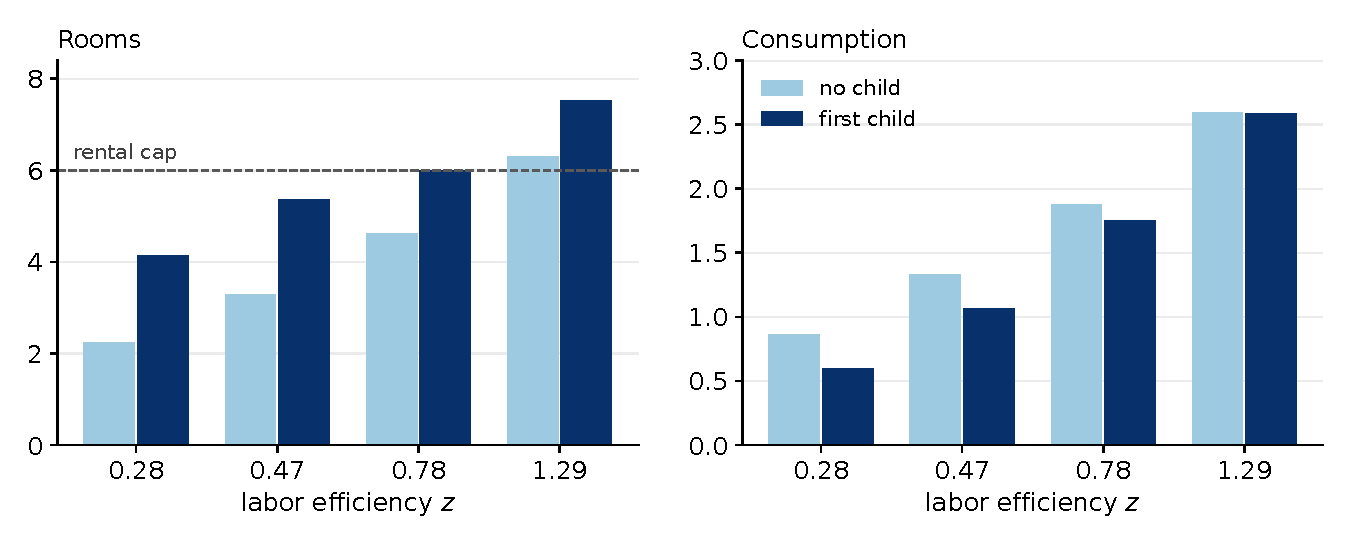
\includegraphics[width=\textwidth,height=0.55\textheight,keepaspectratio]{JMP_slides/frames/cost_of_a_first_child.pdf}
\end{center}
\vspace{-0.8em}
\begin{itemize}\setlength\itemsep{2pt}
\item A first child needs up to two more rooms
\item Renters cannot borrow, so the extra rent cuts consumption, by 31\% at low earnings
\end{itemize}
\end{frame}
